\documentclass{article}

\usepackage{lmodern}
\usepackage[english]{babel}
\usepackage{color}

\usepackage{fontspec}
\defaultfontfeatures{Ligatures=TeX}

\usepackage{listings}
\usepackage{float}
\usepackage{hyperref}

\usepackage{graphicx}
\graphicspath{{assets/}}

\usepackage[
  style   = numeric,
  sorting = none,
]{biblatex}
\bibliography{paper}

% http://latexcolor.com
\definecolor{amaranth}{rgb}{0.9, 0.17, 0.31}
\definecolor{gray}{rgb}{0.5, 0.5, 0.5}
\definecolor{ceruleanblue}{rgb}{0.16, 0.32, 0.75}
\definecolor{green(ncs)}{rgb}{0.0, 0.62, 0.42}
\definecolor{auburn}{rgb}{0.43, 0.21, 0.1}

\lstset {
  basicstyle        = \normalfont\ttfamily\small,
  breakatwhitespace = false,
  breaklines        = true,
  showspaces        = false,
  showstringspaces  = false,
  showtabs          = false,
  tabsize           = 2
}

\lstset {
  commentstyle      = \color{gray},
  keywordstyle      = \color{blue},
  stringstyle       = \color{green(ncs)}
}

\title{Analysing commit messages}

\begin{document}
  \maketitle

  \section{Introduction}
\label{sec:introduction}

With the rise of open source software, more and more big corporations
incorporate free software in their stack. This also means that the amount of
meaningful software that is available online on platforms like GitHub
\cite{github}, is ever increasing. GitHub, as the name already suggest, offers
the ability to host Git repositories. Git is a distributed version control
system \cite{git}. In this paper an effort has been made to analyse Git commits
and gather information on their intended basic operation by looking at the
message of the commit. Therefore repositories of the top 10 most wanted
programming language according to \cite{so-survey} have been investigated. To
get a more accurate representation of each language, 100000 commits have been
chosen. To enhance diversity, only the last 10000 commits of each selected
repository were used.  The analysis has been done in Python.


  \section{Related Work}
\label{sec:related-work}

The idea of classifying commits is based on the concept of labelling
messages with a specific tag. Already labelled commit messages can be
seen as correctly labelled, as the author is unlikely to label their commit
incorrectly. Furthermore we have many authors for our selection of
messages essentially giving us a collaborative labelling approach,
which has already been well researched to result in a representative
dataset \cite{Golder2006}.

While this study only focuses on the lexicographical analysis of the
commit message, we can also infer a lot of information about the meaning
of a commit through other factors like code changes. From this we can
conclude if a commit only fixes some mistakes or introduces completely
new features by analysing its size \cite{Hindle2008}.

We can also use commit messages to infer information about the
changes themselves, which can be especially useful when doing version
control analysis. Automatically tagging and understanding the idea
or reason behind a commit can reduce the effort of others working
with the same codebase. Correct labelling can reduce the effort
of filtering commits relevant to a certain part of the codebase or
make it easier for developers to find relevant changes by other
contributors \cite{Mockus2000}. An example would be to check if
a commit introduces a fix for an issue. For some repositories
it was determined that the amount of changes directly contributes
to the likelihood of being a fix, \cite{Sliwerski2005}. However,
this might not be true for all codebases in general.

While gathering information using all metrics of a commit can yield
good results, only analysing the message itself is less trivial.
Using many different repositories for commit resources also greatly
increases diversity, which can ultimately lead to lower accuracy
of a predictive model \cite{Mockus2000,Santos2020}.

The most important factor in commit classification is the selection
of labels, as they can greatly influence the prediction results.
However, applying too many labels might result in a very complex
classification problem, where commits cannot be properly fitted
to a single category ultimately resulting in wrong predictions
\cite{Santos2020}.

  \section{Methodology}
\label{sec:methodology}

As already alluded to in \autoref{sec:introduction}, the goal of the project is to
collect and analyse commit messages. To achieve this, repositories of the top 10 most
wanted languages, according to a yearly StackOverflow survey (seen in
\autoref{fig:wanted_languages}), were used. This list was used as a reference, since it
has a great assortment of languages that are in high demand and also relevant
in today's development climate. The languages in question are:

\begin{figure}[H]
  \centering
  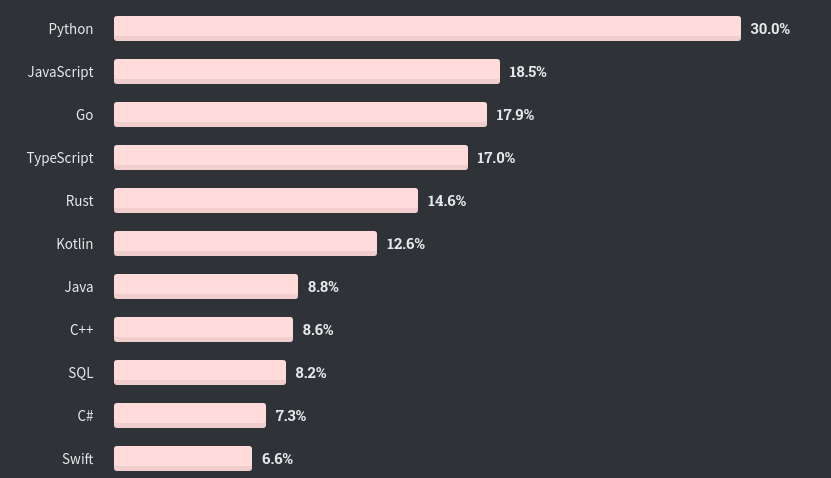
\includegraphics[width=\textwidth]{wanted_languages.png}
  \caption{Top 10 Most Wanted Languages \cite{so-survey}}
  \label{fig:wanted_languages}
\end{figure}

It has to be noted that not all languages depicted in \autoref{fig:wanted_languages}
have been chosen since SQL is a query language and not considered a general
programming language. We therefore excluded SQL since
it is not suited to be used as the main language for a repository.
Swift has been included as the \whitelist{10th} language instead.
Regardless of the percentages seen in \autoref{fig:wanted_languages}, 100000 commits of each
language have been considered for the final set, where 10000 is the maximum per
repository. To further diversify the results, a limit has been imposed regarding
the amount of commits per author. This limit has been set to 100, since commit
messages by the same author are very likely to use a similar order of words,
even across different repositories. The authors are distinguished by their
e-mail addresses.

The language of choice for the programming part of the dataset retrieval
is Python. Python is well suited for this project as it has rich support for
natural language processing related tasks. Additionally the language is great
for quick prototyping of ideas and with the help of tools like Jupyter
Notebook, documents with graphs and text can be created with little effort. Especially
during the scraping process, the library PyGithub was put to good use. PyGithub
is a Python library that offers typed interactions with the GitHub API v3
\cite{pygithub}. The results of the fetching process are furthermore cached in
one CSV file per language. As those files used the same format and headers, they
can easily be combined into one large file for convenience. However, the language
is also included as an additional column in order to not lose this information.

The dataset was analysed using the NLTK library \cite{nltk} and Python.
The library was used to generate different word distributions and process
the messages themselves.

Since some repositories contain commits that are already tagged with some label,
regular expressions were used to filter a subset of those commits.
This subset was used to test a basic classification approach. The idea is to
determine how good a simple approach, only based on text analysis, actually is.

For the classification approach, the logistic regression implementation from
the Python module sklearn \cite{sklearn} was used. A subset of all extracted
tags were used to generate a common set of labels.
The feature vectors for the logistic regression were created by tokenising the
commit messages. The validation of the classifier was done using
10-fold cross-validation.

  \section{Implementation}
\label{sec:implementation}

The implementation itself is comprised of three parts:

\begin{itemize}
  \item Scraping
  \item Tagging
  \item Training/Testing
\end{itemize}

\subsection{Scraping}

The scraping process is a curious case since it was problematic to some extent.
More in that regard can be found in \autoref{sec:challenges}. The basic idea
of the scraping process was to fetch repositories and their commits from
GitHub. This was done with the help of PyGithub. The code itself for the
process of repository gathering is rather simple. A basic array with all
languages was defined as seen in \autoref{lst:languages}, which is then used to
iterate over and actually search for repositories for the corresponding language
with the specific GitHub query syntax as seen in \autoref{lst:query}.

\begin{lstlisting}[language=python, label={lst:languages}, caption={Array of all languages for scraping}]
languages = [
  'python',
  'javascript',
  'go',
  'typescript',
  'rust',
  'kotlin',
  'java',
  'c++',
  'c#',
  'swift',
]
\end{lstlisting}

\begin{lstlisting}[language=python, label={lst:query}, caption={GitHub query syntax}]
g.search_repositories(
  query=f'language:{language}', sort='stars', order='desc'
)
\end{lstlisting}

This then yields all repositories sorted by stars in descending order.
Stars is a metric on GitHub to show a repository's popularity. Each star
represents a user on GitHub who has starred this repository. Counters keep track of
per-author (100), per-repository (10000) and global (1000000) commit limits.
This means that at least 10 repositories are per per language. When the
\whitelist{100000th} commit is reached, repositories for the next language will
be fetched. Because the process of scraping is time and space intensive, the
results are cached. Per language, one CSV file is created. The file consists of
rows with four columns:

\begin{itemize}
  \item repository
  \item language
  \item author
  \item message
\end{itemize}

With this structure, all important information is included in the file which is
essential for further processing. An example excerpt of one file can be seen in
\autoref{lst:csv}.

\begin{lstlisting}[language=xml, label={lst:csv}, caption={Excerpt of \texttt{typescript.csv} with commits from the repository \texttt{microsoft/vscode}}]
repository,language,author,message
microsoft/vscode,typescript,roblourens@gmail.com,"Fix #126087"
microsoft/vscode,typescript,penn.lv@gmail.com,":notebook: differenciate editor focus and list view focus"
microsoft/vscode,typescript,me@tylerleonhardt.com,"always hide quickinput on iPad when focus is lost fixes #125284"
microsoft/vscode,typescript,connor@peet.io,"fix: use inline sourcemaps in watch task"
microsoft/vscode,typescript,alexdima@microsoft.com,"update `monaco.d.ts`"
\end{lstlisting}

\subsection{Tagging}

The next step is to tag commits. We distinguish between two categories of tagged
commits:

\begin{itemize}
  \item Conventional Commits \cite{conventionalcommits}
  \item Gitmoji \cite{gitmoji}
\end{itemize}

A specific regular expression for each category has to be matched in order to
tag the commit. The lookup in case of a match is done by searching for the
specific tag in a dictionary. Gitmoji commits are mapped to follow the same naming
as Conventional Commits using the lookup table seen in \autoref{lst:gitmoji_map}.
Commits which follow the Conventional Commits format are mapped using \autoref{lst:tag_map}.
In the end, all commits which are tagged following the Angular Commit Message
Guidelines \cite{angular_guidelines} are treated as “known tags” and filtered.
In addition to adding a tag to a commit, the tag is also removed from the original
commit message.

\begin{lstlisting}[language=python, label={lst:gitmoji_map}, caption={Dictionary for Gitmoji mappings}]
gitmoji_mappings = {
  ':memo:':     'docs',     # Documentation
  ':zap:':      'perf',     # Performance
  ':fire:':     'remove',   # Removal
  ':sparkles:': 'feat',     # Feature
  ':bug:':      'fix',      # Bug Fix
  ':recycle:':  'refactor', # Refactor Code
  ...
}
\end{lstlisting}

\begin{lstlisting}[language=python, label={lst:tag_map}, caption={Dictionary for conventional tag mappings}]
tag_mappings = {
  'bug':           'fix',
  'testing':       'test',
  'documentation': 'docs',
  'feature':       'feat',
  'gui':           'ui',
  ...
}
\end{lstlisting}

\subsection{Training \& Testing}

In order to properly train and test the dataset, some filtering has to be done.
With distinct regular expressions common message patterns are filtered from
the commit message. With \lstinline{#\d+}, pull request or issue numbers
are normalised, since they start with a \# and end with a number. Version
numbers can also exacerbate tokenisation and therefore the simple regular
expression \lstinline{\b\d+(\.\d+)+\b} takes care of basic version notations
that are common on GitHub. Email addresses and URLs in general also make
tokenisation more difficult. Therefore, both of those patterns are also
removed.

The next step is then to encode the tags. This can be done with the
\textit{LabelEncoder} from \textit{sklearn}. The \textit{sklearn} library also
offers a \textit{CountVectorizer} with which text documents can be converted
into token counts. The actual training/testing process is done using a
10-fold cross validation which splits the data and yields train and test
indices with which the train and test data can be defined. Both datasets are
then used within the logistic regression to get the final results.

  \section{Results}
\label{sec:results}

For evaluating our dataset generation, we first collected commits without any limits imposed on commits from a single author. We later added a per-author limit in order to avoid bias being introduced by including a vast amount of commits from a single author.

\autoref{fig:total_vs_tagged_with_limit} shows that around 25000 commits (~2.5\%) out of a total of 1000000 commits are tagged when limiting the number of commits per author to 100. Without this limit, the number of tagged commits slightly increases to about 35000 commits (~3.5\%) out of 1000000. Overall, we see that with or without limit, the number of tagged commits remains relatively small compared to the total number of commits.

\begin{figure}[H]
  \centering
  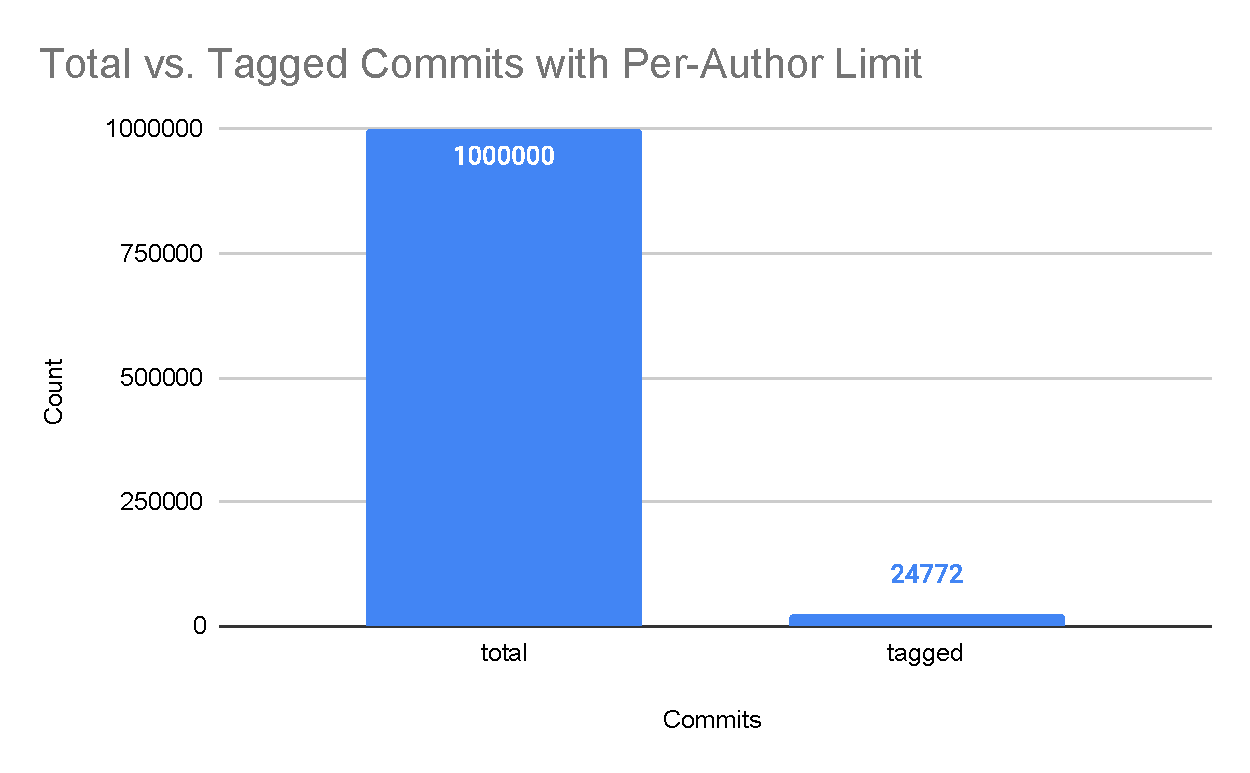
\includegraphics[width=\textwidth]{total-vs-tagged-commits-with-author-limit.pdf}
  \caption{Total vs. Tagged Commits with Per-Author Limit}
  \label{fig:total_vs_tagged_with_limit}
\end{figure}

\begin{figure}[H]
  \centering
  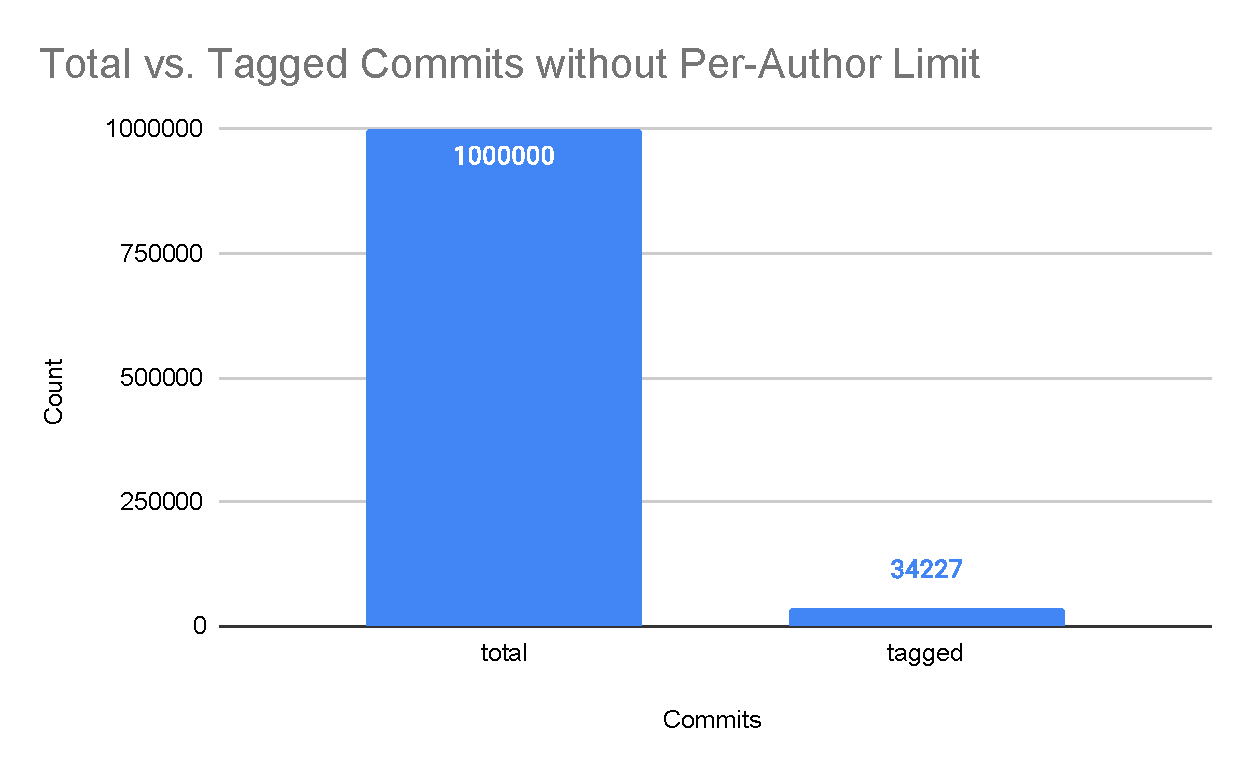
\includegraphics[width=\textwidth]{total-vs-tagged-commits-without-author-limit.pdf}
  \caption{Total vs. Tagged Commits without Per-Author Limit}
  \label{fig:total_vs_tagged_without_limit}
\end{figure}

In \autoref{fig:tag_dist_with_limit} and \autoref{fig:tag_dist_without_limit}, we can see the distribution of commit tags with and without the mentioned per-author limit, respectively. When comparing both graphs, we can see that without a per-author commit limit, the number of commits tagged with “chore” almost doubles while commits tagged with “feat” stay more or less the same. This is likely due to commits being authored by bots, which mainly applies to automatic maintenance tasks, i.e. chores.

\begin{figure}[H]
  \centering
  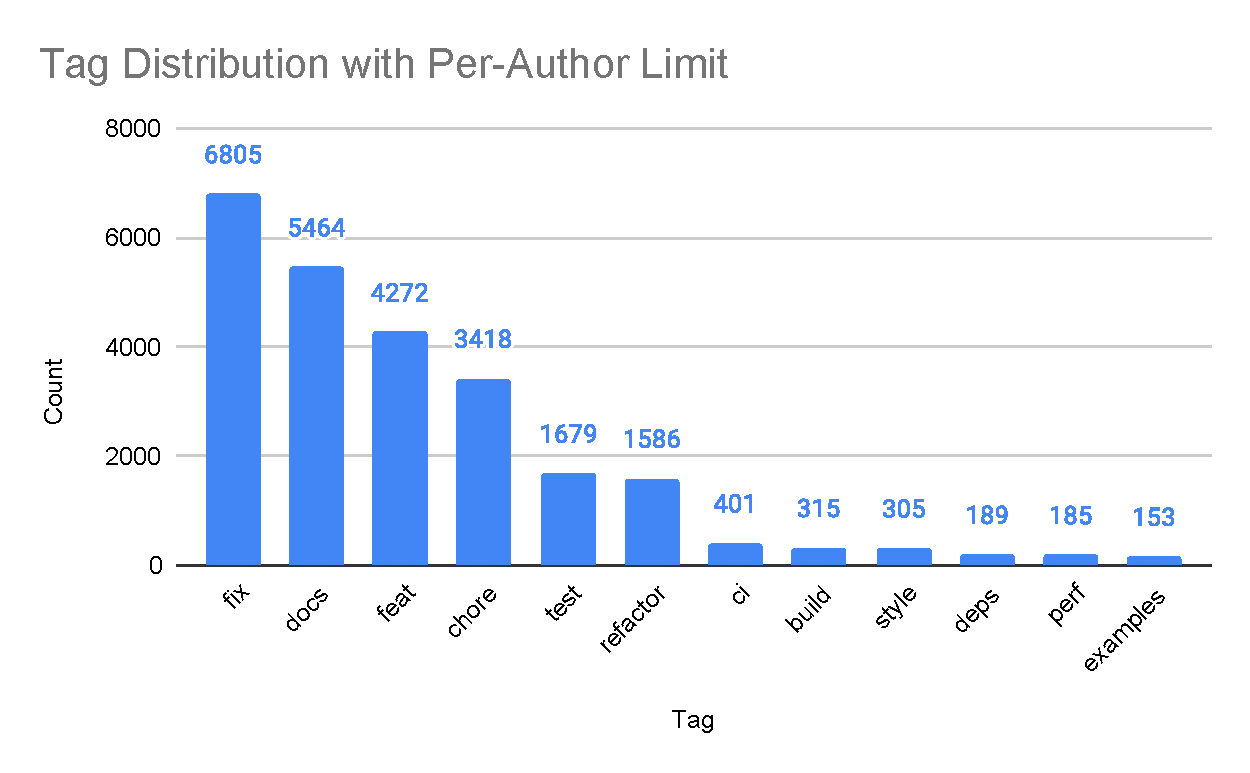
\includegraphics[width=\textwidth]{tag-distribution-with-author-limit.pdf}
  \caption{Tag Distribution with Per-Author Limit}
  \label{fig:tag_dist_with_limit}
\end{figure}

\begin{figure}[H]
  \centering
  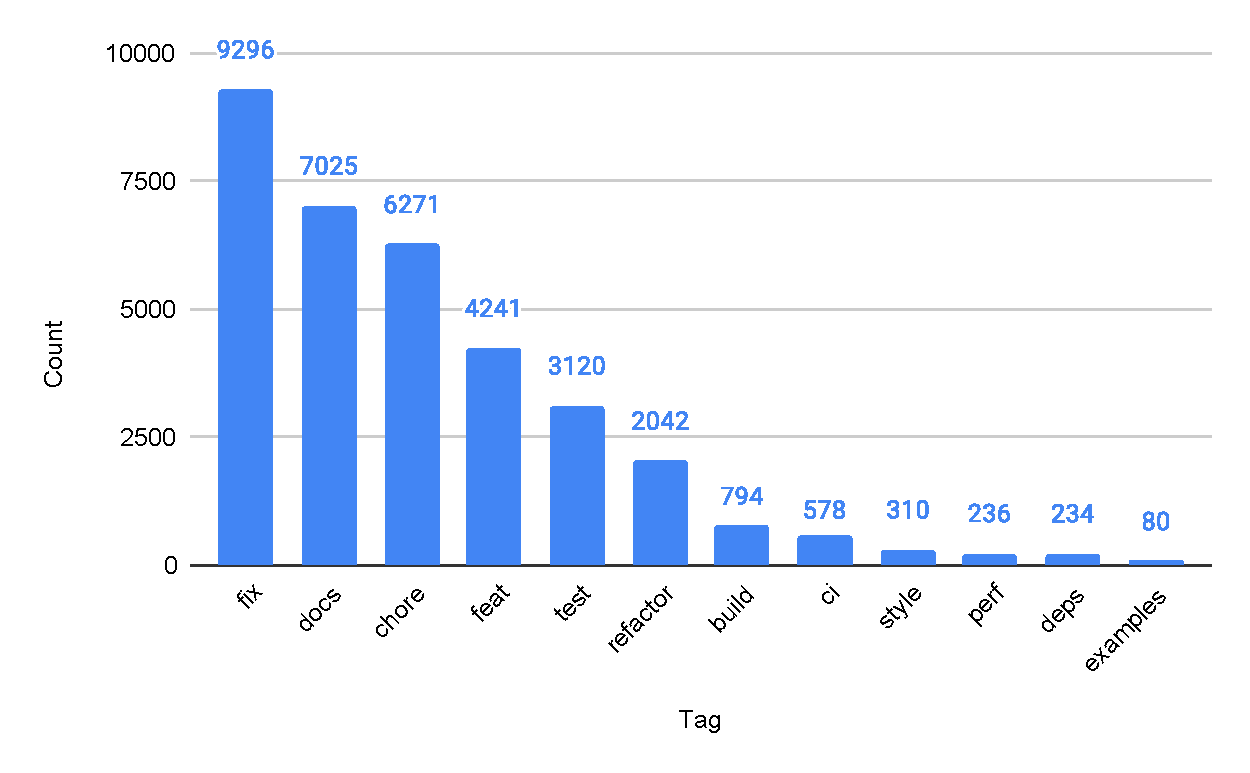
\includegraphics[width=\textwidth]{tag-distribution-without-author-limit.pdf}
  \caption{Tag Distribution without Per-Author Limit}
  \label{fig:tag_dist_without_limit}
\end{figure}

\begin{table}[H]
  \def\arraystretch{1.15}%
  \centering
  \label{fig:unlimited_commits}
  \caption{Unlimited commit messages per author}
  \bigskip
  \begin{tabular}{| l | r |}
    \hline
    Total Accuracy & 0.6517433833828978 \\
    \hline
    Total F1 micro & 0.6517433833828978 \\
    \hline
    Total F1 macro & 0.5371101432803524 \\
    \hline
  \end{tabular}
\end{table}

\begin{table}[H]
  \def\arraystretch{1.15}%
  \centering
  \label{fig:limited_commits}
  \caption{100 commit messages per author}
  \bigskip
  \begin{tabular}{| l | r |}
    \hline
    Total Accuracy & 0.6102058422223566 \\
    \hline
    Total F1 micro & 0.6102058422223566 \\
    \hline
    Total F1 macro & 0.4479298698746271 \\
    \hline
  \end{tabular}
\end{table}


  \section{Challenges}
\label{sec:challenges}

Unfortunately, the project could not be completed without its fair share of
challenges. Starting off with the scraping process which was not as
straightforward as it originally might have seemed. Since all repositories are from
GitHub it was an obvious choice to use the GitHub API, in this case via PyGithub,
for everything regarding scraping. After some testing however, it was clear that
this is not a feasible strategy as the GitHub API imposes a strict request
limit of 5000 requests per hour. Though we can use a single request to get a
repository, getting the messages for all commits requires a separate API
request for each commit. Since we have to go over each commit in
order to get the commit message, 5000 requests are reached in no time with the
goal of 100000 commit messages per language.

Ultimately, rethinking our strategy was the only option. This did not mean that
we had to abandon PyGithub completely as we still use it to query the
repositories. Gathering the commits was only really possible by actually
cloning the repository and going over the commits with the Git command line utility
itself. Usually this is a reasonable way of fetching commits, however
with the amount of repositories we are working with, this was rather cumbersome,
since the disk space requirements were considerable. Once the limits on commits per
author was in place, we had to clone 120GB worth of repositories. This is due to a few
authors having significantly more contributions to a repository than other authors of the
same repository. However this is to be expected as open source project
maintainers often work in a smaller group for a long time duration. Furthermore
each scraping run was also time intensive considering the fact that each
repository had to be cloned and processed.

Another challenge was the selection of repositories itself. In the end we settled
on sorting them by stars. However this is not necessarily a proper metric to
determine popularity. Since every user can star an unlimited amount of
repositories, the possibility of stars contributed by fake accounts cannot be
excluded. Furthermore, users might star a repository for different reasons like
appreciation or bookmarking. It would probably be more accurate to use a
combination of stars, forks and watchers. Our goal however is to collect a set
of commits, which is representative of the whole set of commits on GitHub.
Since we have a great variety of repositories for each language, we can
accept a weaker indication of popularity.

\end{document}
